%% -----------------------------------------

%% Vorlesungsmitschrift (Kapitel 4)

%% an der Uni Regensburg, gelesen von Christian Back

%% -----------------------------------------


\chapter{Elektromagnetische Wellen an Grenzflächen}
\section{Randbedingungen der elektromagnetischen Welle}
Wir wollen jetzt Wellenausbreitung in inhomogenen Medien beschreiben,
z.\,B. den Übergang von Medium~1 nach Medium~2, also einer
Grenzfläche.

\paragraph{Randbedingungen der MWGl.:} Die Tangentialkomponenten von
$\vecE$ und $\vecH=\fracone{\muo\mu_r}\vecB$ sind stetig. Die
Normalkomponenten von $\vecD=\epso\eps_r\vecE$ und $\vecB$ sind
ebenfalls stetig (Erinnerung: Für isotrope, isolierende, nicht
magnetische Medien gilt $\mu_r\eqqcolon\mu=1$).
\paragraph{einfachster Fall:} Wir betrachten zwei homogene Medien mit
Brechungsindex $n_e$ (einfallender Strahl) und $n_t$ (transmittierte
Welle).
% 
%% Skizze zu Reflexion
% 
Der Winkel $\alpha$ liegt zwischen $\veck_e$ und $\vece_y$
bzw. zwischen $\veck_t$ und $\vece_y$. Wir nehmen an, dass es eine
fest vorgegebene einlaufende Welle ist.
\begin{align*}
  \vecE_e &= \vecE_{0,e}\cos(\omega_et-\veck_e\vecr)
            =\vecE_{0,e}(\phi_e(\vecr,t))\\
  \vecE_r &= \vecE_{0,r}\cos(\omega_rt - \veck_r\vecr+\varphi_r)
            =\vecE_{0,r}(\phi_r(\vecr,t))\\
  \vecE_t &= \vecE_{0,t}\cos(\omega_tt - \veck_t\vecr + \varphi_t)
            =\vecE_{0,t}(\phi_t(\vecr,t))
\end{align*}
Die Wellenvektoren $\veck_e$, $\veck_r$ und $\veck_t$ müssen die%
\nomenclature{$\veck_e$}{Wellenvektor der einlaufenden Welle}%
\nomenclature{$\veck_t$}{Wellenvektor der transmittierten Welle}%
\nomenclature{$\veck_r$}{Wellenvektor der reflektierten Welle}
Dispersionsrelationen im jeweiligen Medium erfüllen. Die
\emph{Phasenfaktoren}\index{Phasenfaktoren}
$\varphi_r$, $\varphi_t$%
\nomenclature{$\varphi_r$}{Phasenfaktor der reflektierten Welle;
  bestimmt Phasenverschiebung zur einlaufenden Welle}%
\nomenclature{$\varphi_t$}{Phasenfaktor der transmittierten Welle;
  bestimmt Phasenverschiebung zur einlaufenden Welle} 
bestimmen die Phasenlage relativ zur einlaufenden Welle.

% -------------------

\section{Reflexions- und Brechungsgesetz}
Die Stetigkeit der Tangentialkomponente des elektrischen Feldes an der
Grenzfläche ist wichtig für den Wellenverlauf.
Daher muss man die Randbedingung annehmen, dass die $x$- und die
$z$-Komponente von $\vecE$ und $\vecH$ stetig sein müssen.
Z.\,B. ist für
\begin{align*}
  E_{0_{e_x}} \cos(\phi_e(\vecr,t)) 
  +  E_{0_{r_x}} \cos(\phi_r(\vecr,t)) 
  &=   E_{0_{t_x}} \cos(\phi_t(\vecr,t)) \\
  E_{0_{e_z}} \cos(\phi_e(\vecr,t)) 
  +  E_{0_{r_z}} \cos(\phi_r(\vecr,t)) 
  &=   E_{0_{t_z}} \cos(\phi_t(\vecr,t)) \\
\end{align*}
die notwendige Bedingung, dass für alle $t$ und alle $\vecr$
mit $y=0$ gilt
\begin{gather*}
  \phi_e(\vecr, t) = \phi_r(\vecr,t) = \phi_t(\vecr, t) 
  \qquad\text{bzw.}\\
  \omega_et- \veck_e\vecr = \omega_rt- \veck_r\vecr = \omega_tt- \veck_t\vecr
\end{gather*}
Diese ist nur erfüllbar, wenn folgendes gilt
\begin{itemize}
\item $\omega_e=\omega_r=\omega_t$.\\
  \red{Achtung:} Es ist eine Wellenlängenänderung möglich.
\item Die Ebenengleichungen
  \begin{align*}
    \veck_e\vecr &= \veck_r\vecr \quad\text{bzw.} \quad(\veck_e-\veck_r)\vecr=0\\
    \veck_e\vecr &= \veck_t\vecr \quad\text{bzw.} \quad(\veck_e-\veck_t)\vecr=0
  \end{align*}
  D.\,h. die Vektoren $(\veck_e-\veck_r)$
  und $(\veck_e-\veck_t)$ müssen senkrecht auf der Ebene $y=0$ stehen.
\end{itemize}
Daraus folgt, dass die Komponenten $\veck_e$ und $\veck_r$ parallel
zur Grenzfläche gleich sein müssen:
\begin{gather*}
  \veck_e = \veck_r
\end{gather*}
Setzt man hier nun die Dispersionsrelation 
$\veck^2 = \frac{n^2\omega^2}{c^2}$ ein, erhält man
$k_{e_G} = \frac{\omega n_e}{c}\sin\alpha = k_{r_G} 
= \frac{\omega n_e}{c}\sin\alpha'$, umgeschrieben das
\emph{Reflexionsgesetz}\index{Reflexionsgesetz}
\begin{gather*}
  \sin\alpha = \sin\alpha'
\end{gather*}
Die Oberflächennormalen $\vece_y$ und $\veck_e$ spannen die
Einfallsebene auf, in der auch $\veck_r$ liegen muss (d.\,h. keine
Seitwärtsreflexion).

\paragraph{Transmittierter Strahl} Für den transmittierten Strahl
erhält man analog $\veck_{e_r} = \veck_{t_G}$ und daraus wieder mit
der Dispersionsrelation
$k_{e_G} = \frac{\omega n_e}{c}\sin\alpha 
= k_{t_G} =  \frac{\omega n_t}{c}\sin\beta$, also das sog.
\emph{Snellins'sche  Brechungsgesetz}%
\index{Brechungsgesetz!Snellins'sches Brechungsgesetz}
\begin{gather}
  n_e\sin\alpha = n_t\sin\beta
  \label{brechungsgesetz}
\end{gather}
%% IMAGE MISSING

Es gilt anschaulich
\begin{description}
\item[$n_e<n_t$] zum Lot hin gebrochen
\item[$n_e>n_t$] vom Lot weg gebrochen
\end{description}
und mit relativem Brechungsindex $n_{et}=\frac{n_e}{n_t}$ lässt sich
\eqref{brechungsgesetz} umformen zu
\begin{gather*}
  \sin\alpha = n_{et} \sin\beta
\end{gather*}

% ---------------

\section{Die Fresnel'schen Formeln}
Die in diesem Kapitel behandelten 
\emph{Fresnel'schen Formeln}\index{Fresnel'sche Formeln}
beschreiben den Reflexionsgrad einer Grenzfläche.
Dieser hängt von der \emph{Polarisation} ab.

\subsection{Linear Polarisiertes Licht}\label{4.3.1}%
\index{Polarisation!linear polarisiertes Licht}
Es sei $\vecE\bot\vecB$ und $\vecE,\vecB\bot\veck$.
Definiere $\veck= (0,0,k_z)$, dann liegt $\vecE$ in der $x$-$y$-Ebene
mit
\begin{gather*}
  \vecE = \vecE_x + \vecE_y 
  =\begin{pmatrix}
    E_{x,0} \cos(k_z z - \omega t)\phantom{~+ \varphi}\\
    E_{y,0} \cos(k_z z - \omega t + \varphi)\\
    0
  \end{pmatrix}
\end{gather*}
Man sieht, dass eine Phasendifferenz zwischen $E_x$ und $E_y$
möglich ist. Für $\phi=0$ bzw. $\phi=\pm m\pi$ ($m\in\mathds{N}$) gilt
\begin{gather*}
  \vecE = \begin{pmatrix} E_{x,0}\\E_{y,0}\\0 \end{pmatrix}
  \cos(k_zz - \omega t)
  = \vecE_0  \cos(k_zz - \omega t)
\end{gather*}
Die Richtung von $\vecE_0$ ist nicht zeitabhängig.

% ---

\subsection{Zirkular polarisiertes Licht}\label{4.3.2}%
\index{Polarisation!zirkular polarisiertes Licht}
Zirkular polarisiertes Licht ist der Spezialfall $E_{x,0} = E_{y,0} = E_0$
und $\varphi = \frac{\pi}{2} + m\pi$ (wieder $m\in\mathds{N}$), in
Formel
\begin{gather*}
  \vecE = E_0\begin{pmatrix} 
    \cos(k_zz - \omega t)\phantom{~+ \frac{\pi}{2} + m\pi}\\
    \cos(k_zz - \omega t + \frac{\pi}{2} + m\pi)\\
    0 
  \end{pmatrix}
  = E_0\begin{pmatrix} 
    \phantom{\pm}\cos(k_zz - \omega t)\\
    \pm\sin(k_zz - \omega t)\\
    0 
  \end{pmatrix}
\end{gather*}
Hier ist der Betrag der Feldstärke zeitlich konstant und der
$\vecE$-Vektor beschreibt eine Helixbahn (s. Folien), während $m$ den
Drehsinn bestimmt. Die Unterscheidung zwischen rechts und links zirkular ist:
\begin{description}
\item[rechts zirkulares Licht] Blick zur Lichtquelle,
  $\vecE$ rotiert im Uhrzeigersinn
\item[links zirkulares Licht] Blick zur Lichtquelle,
  $\vecE$ rotiert gegen den Uhrzeigersinn
\end{description}

% ---

\subsection{Elliptisch polarisiertes Licht}\label{4.3.3}%
\index{Polarisation!elliptisch polarisiertes Licht}
Hier gilt $E_{x,0} \neq E_{y,0}$ und $\varphi$ ist beliebig.
Dann Beschreibt der $\vecE$-Vektor eine Ellipse in $x$-$y$-Richtung.

\subsection{Fresnel'sche Formeln}
Bisher wurden nur die Phase und damit die Ausbreitungsvektoren
betrachtet.
Jetzt betrachten wir die Amplituden.
Dazu spaltet man die Felder in Komponenten parallel und senkrecht zur
Einfallsebene auf:
\begin{description}
\item[$E_s$ bzw. $E_\bot$] Feldvektor schwingt senkrecht zur
  Einfallsebene; $E_s$ ist automatisch tangential zur Grenzfläche
\item[$E_p$ bzw. $E_\parallel$] Feldvektor schwingt in der Einfallsebene
\end{description}

% ---

\subsection{Senkrechter Lichteinfall}
Wir nehmen für senkrechten Lichteinfall folgende Randbedingungen für
das elektrische und magnetische Feld an
\begin{align}
  \vecE_{0_e} + \vecE_{0_r} = \vecE_{0_t} \label{randbed1}\\
  \vecH_{0_e} + \vecH_{0_r} = \vecH_{0_t} \label{randbed2}
\end{align}
Verwendet man die MWGl
$\vecna\times\vecE = -\dif[\vecB]{t} = -\muo\mu\dif[\vecH]{t}$
und setzt alles in die ebene Welle ein, erhält man
\begin{gather*}
  \vecE(\vecr,t) = \vecE_0 e^{i(\veck\vecr-\omega t)} 
  \qquad{und}\qquad
  \vecB(\vecr,t) = \vecB_0 e^{i(\veck\vecr-\omega t)} 
\end{gather*}
sowie
\begin{align*}
  \begin{pmatrix}
    \dif[E_{0,z}e^{i(\veck\vecr-\omega t)}]{y}
    - \dif[E_{0,y}e^{i(\veck\vecr-\omega t)}]{z}\\
    \dif[E_{0,x}e^{i(\veck\vecr-\omega t)}]{z}
    - \dif[E_{0,z}e^{i(\veck\vecr-\omega t)}]{x}\\
    \dif[E_{0,y}e^{i(\veck\vecr-\omega t)}]{x}
    - \dif[E_{0,x}e^{i(\veck\vecr-\omega t)}]{y}\\
  \end{pmatrix}
&= - \dif[\vecB_0e^{i(\veck\vecr-\omega t)}]{t}\\
  \Longleftrightarrow
  \begin{pmatrix}
    E_{0,z}\cdot ik_y - E_{0,y} \cdot ik_z\\
    E_{0,x}\cdot ik_z - E_{0,z} \cdot ik_x\\
    E_{0,y}\cdot ik_x - E_{0,x} \cdot ik_y
  \end{pmatrix}
& = -\vecB_0\cdot (-i\omega)
\end{align*}
Also
\begin{align}\nonumber
  \veck\times\vecE_0 &= \omega\vecB \qquad\qquad\text{bzw.}\\
  \vecB_0 &= \frac{1}{\omega}(\veck\times\vecE_0) \label{randbed3}
\end{align}
Setze \eqref{randbed3} in \eqref{randbed2} ein und erhalte
\begin{gather*}
  \frac{1}{\omega}(\veck_e\times\vecE_{0,e}) 
  +   \frac{1}{\omega}(\veck_r\times\vecE_{0,r})
  = \frac{1}{\omega}(\veck_t\times\vecE_{0,t}) 
\end{gather*}
da $\veck\bot\vecE$ und $\veck_e = -\veck_r$, 
$\veck_t = \frac{n_t}{n_e}\veck_e$. Daraus erhält man
\begin{gather*}
  n_e\vecE_{0,e} -   n_r\vecE_{0,r} =   n_t\vecE_{0,t}
\end{gather*}
Eliminiere $\vecE_{0,t}$ durch Einsetzen von \eqref{randbed1}
\begin{align*}
  \vecE_{0,r} &= \frac{n_e-n_t}{n_e+n_t} \vecE_{0,e} = r\vecE_{0,e}
  &r &= \frac{n_e-n_t}{n_e+n_t} 
  &&\text{(Reflexionskoeffizient)}\\
  \vecE_{0,t} &= \frac{2n_e}{n_e+n_t} \vecE_{0,e} = t\vecE_{0,e}
  &r &= \frac{2n_e}{n_e+n_t} 
  &&\text{(Transmissionskoeffizient)}
\end{align*}%
\index{Reflexionskoeffizient}%
\nomenclature{$r$}{Reflexionskoeffizient;
  $r=\frac{n_e-n_t}{n_e+n_t}$}%
\index{Transmissionskoeffizient}%
\nomenclature{$t$}{Transmissionskoeffizient; $t=\frac{2n_e}{n_e+n_t}$}%

% -----------------
% 05.11.2015
% -----------------
\marginpar{05.11.2015}

\begin{description}
\item[$n_e>n_t$:] Wenn Licht von optisch dichteren in ein optisch dünneres
  Medium übergeht, ist der Reflexionskoeffizient größer null. 
  Daraus folgt, dass $\vecE_{0r}$ und $\vecE_{0e}$ in die gleiche
  Richtung zeigen und die Wellen an der Grenzschicht in Phase sind. 
\item[$n_e<n_t$:] Wenn Licht aus einem optisch dünneren in ein optisch dichteres
  Medium übergeht, wird der Reflexionskoeffizient kleiner Null und
  $\vecE_{0r}$ und $\vecE_{0e}$ zeigen in antiparallele Richtungen
  Außerdem liegt bei der Reflexion ein Phasensprung von $\pi$ vor,
  bei Transmission aber nicht.
\end{description}
Da die reflektierte Intensität nur proportional zu
$|\vecE|^2$ ist, spielt der Phasenfaktor keine Rolle.

\minisec{Reflexionsgrad%
\nomenclature{$R$}{Reflexionsgrad}%
\index{Reflexionsgrad}
der Intensität}
\begin{gather*}
  R = \frac{I_r}{I_e}
  =\left( \frac{n_e-n_t}{n_e+n_t} \right)^2
  =\left( \frac{n_{et}-1}{n_{et}+1} \right)^2
  =\left( \frac{1-n_{te}}{1+n_{te}} \right)^2
\end{gather*}
Der Reflexionsgrad ist unabhängig davon, von welcher Seite das Licht
einfällt. Er hängt allein von der Änderung des relativen
Brechungsindex ab. Wird das Licht aber absorbiert, wird der
Reflexionskoeffizient komplex und kann geschrieben werden als
\begin{align*}
  R=\vert r\vert^2=rr^*
\end{align*}
\paragraph{Beispiel:}
\begin{center}
  \begin{tabular}{lll}
    \emph{Übergang} & \emph{relativer Brechungsindex} & \emph{Reflexion in \%}\\
    Luft -- Glas & \num{1.5} & \SI{4}{\percent} \\
    Luft -- Diamant & \num{2.41} & \SI{17}{\percent}
  \end{tabular}
\end{center}

\subsection[Beliebige Einfallswinkel]{Beliebige Einfallswinkel $\alpha$}
Zunächst betrachten wir ein $\vecE$-Feld, das parallel zur
Einfallsebene schwingt und p"=polarisiert (d.\,h. parallel zur Einfallebene)
ist. Im Folgenden werden die Tangentialkomponenten mit dem Index~$T$
versehen und die Normalkomponenten mit dem Index~$N$. Betrachte außerdem
noch die Setigkeitsbedingungen für $\vecE$ und
$\vecD=\epso\eps\vecE$.
\begin{align*}
  E_{eN} &= E_e\sin\alpha
  &E_{tN} &= E_t\sin\beta
  &E_{rN} &= E_r\sin\alpha\\
  E_{eT} &= E_e\cos\alpha
  &E_{tT} &= E_t\cos\beta
  &E_{rT} &= -E_r\cos\alpha
\end{align*}
% ------------------------------------------------------------------------------
% Hab mir hier die Herleitung gespart oder sollen wir sie doch noch
% mit rein nehmen? 
% ------------------------------------------------------------------------------
Mit Hilfe der Stetigkeitsbedingungen und der Snellschen Formel,
erhalten wir daraus die 
\emph{Fresnelschen Formeln}\index{Fresnelsche Formeln}, 
Wobei $r_p$ der Reflexionskoeffizient für p"=polarisiertes Licht ist. 
\begin{align}
  r_{\parallel} 
  &= r_p
    = \frac
    {n_t\cos\alpha - n_e\cos\beta}
    {n_t\cos\alpha + n_e\cos\beta}
    = \frac
    {\tan(\alpha - \beta)}
    {\tan(\alpha + \beta)}\label{FF1}\\
  r_{\bot}
  &=r_s
    = \frac
    {n_e\cos\alpha - n_t\cos\beta}
    {n_e\cos\alpha + n_t\cos\beta}
    = -\frac
    {\sin(\alpha - \beta)}
    {\sin(\alpha + \beta)}\label{FF2}
\end{align}
Die Amplituden der reflektierten $\vecE$-Felder erhält man durch
Multiplikation der Amplituden des emittierten $\vecE$-Felder mit den
Reflexionskoeffizienten.

\minisec{Transmittierte Leistung $P_t$%
\nomenclature{$P_t$}{transmittierte Leistung}%
\index{transmittierte Leistung} 
und Intensität $I_t$%
\nomenclature{$I_t$}{transmittierte Intensität}%
\index{transmittierte Intensität}}
Wenn man nicht direkt an den Amplituden sondern an der
Leistung interessiert ist, kann man diese auch über den
Transmissionsgrad $T^P=\frac{P_t}{P_e}$ 
(bzw. bei der Intensität
$T^{I}=\frac{I_t}{I_e}$%
\index{Transmissionsgrad}%
\nomenclature{$T^P$}{Transmissionsgrad der Leistung; 
  $T^P=\frac{P_t}{P_e}$}%
\nomenclature{$T^I$}{Transmissionsgrad der Intensität;
  $T^{I}=\frac{I_t}{I_e}$})
berechnen. Aufgrund der Energieerhaltung gilt $P_e=P_r+P_t$ und man
erhält
\begin{gather*}
  T_{\parallel}^P = 1-\vert r_{\parallel}\vert^2
  \qquad\text{sowie}\qquad
  T_{\bot}^P = 1-\vert r_{\bot}\vert^2
\end{gather*}
Für die Berechnung der Intensität ist allerdings die Änderung der
Fläche zu berücksichtigen, da sich die Ausdehnung des Lichtstrahls auf
der Einfallebene und im transmittierten Strahl ändert.
\begin{align*}
  d^\prime &= \frac{d}{\cos\alpha}
  &d_t &= d^\prime\cos\beta 	
\end{align*}
Nun kann man folgende Gleichungen formulieren
\begin{align*}
  T^p &=\frac{P_t}{P_e}
        =\frac{I_t A_t}{I_e A_e}
        =\frac{I_t \cos\beta}{I_e\cos\alpha}
        =\frac{n_t |t|^2 \cos\beta}{n_e\cos\alpha}\\
  T^{I}&=\frac{I_t}{I_e}
         =T^P\frac{\cos\alpha}{\cos\beta}
         = |t|^2\frac{n_t}{n_e}
\end{align*}

\subsubsection{Diskussion der Fresnel'schen Formeln: Reflexionsgrad
  bei Lichteinfall aus einem optisch dünnerem Medium}
Ein Beispiel hierfür ist der Übergang von Luft in Gas mit $\frac{n_t}{n_e}=1,5$.
Betrachte nun die Winkelabhängigkeit von $R=\vert r\vert^2$ aus den
Fresnel'schen Formeln \ref{FF1} und \ref{FF2}. 
Bei Erhöhung des Winkels steigt $R_{\bot}$ stetig von \SI{4}{\percent}
bis \SI{100}{\percent} an. 
$R_{\parallel}$ sinkt hingegen anfangs bis zu einem gewissen Winkel
auf Null ab. Dieser Winkel wird auch
\emph{Brewsterwinkel}%
\nomenclature{$\alpha_B$}{Brewsterwinkel; 
  Winkel, bei dem reflektierter und gebrochener Strahl senkrecht
  aufeinander stehen; 
  Winkel vollständiger linearer Polarisierung bei Reflektion;
  $\tan\alpha_B = \frac{n_t}{n_e}$}%
\index{Brewsterwinkel} 
genannt, danach steigt
$R_{\parallel}$ ebenfalls auf die \SI{100}{\percent} an (siehe
Abb.\ref{RefGrad}).
\begin{figure}
  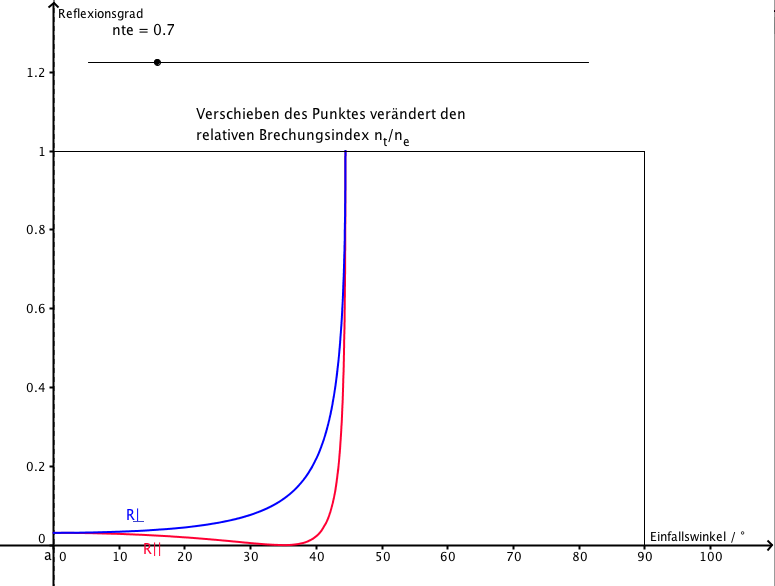
\includegraphics[width=\linewidth]{Bilder/Reflexionsgrad}
  \caption{Reflexionsgrad in Abhängigkeit des Einfallwinkels\label{RefGrad}}
\end{figure}
Der Brewsterwinkel $\alpha_B$ oder auch $\alpha_P$ wird dann erreicht,
wenn der Nenner divergiert, also $\tan(\alpha_B+\beta)=\infty$
bzw. $\alpha+\beta=90\degree$. In diesem Fall stehen der reflektierte
und der gebrochene Strahl aufeinander senkrecht.
Dies lässt sich wie folgt erklären. Man nehme an, dass der
reflektierte Strahl durch einen oszillierenden Dipol mit Dipolmoment
parallel zum $\vecE$-Feld in der Grenzschicht erzeugt wird. Dabei ist
die abgestrahlte Leistung $P(\theta)\propto\sin^2\theta$ und $\theta$
ist der Winkel zwischen Wellenvektor des abgestrahlten Lichts und
Dipolachse. Also wird längs zur Dipolachse ($\theta=0$) kein Licht
abgestrahlt -- $\vecE_{\parallel}$ wird nicht reflektiert. 
\emph{Daraus kann man folgern, dass das Licht vollständig linear
  polarisiert ist.}
Der Brewsterwinkel ergibt sich aus der Formel
\begin{align*}
  \tan\alpha_B &= \frac{n_t}{n_e}
\end{align*}


% -----------------
% 09.11.2015
% -----------------
\marginpar{09.11.2015}

%% Anmerkung letzte Vorlesung
% \begin{align*}
%   E_{eT} &= E_e\cos\alpha\\
%   E_{tT} &= E_t\cos\beta\\
%   E_{rT} &= \mathbf{-} E_r\cos\alpha
% \end{align*}
% \begin{align*}
%   E_{eN} &= E_e\sin\alpha
%   &E_{tN} &= E_t\sin\beta
%   &E_{rN} &= E_r\sin\alpha
% \end{align*}
% \begin{align*}
%   E_{eT} + E_{rT} &= E_{rT}\\
%   \cos\alpha(E_{e}-E_t) &= E_t\cos\beta
% \end{align*}

% 2.
\paragraph{Reflexionsgrad bei Lichteinfall aus optisch dichteren
  Medien}
Wir betrachten $n_e>n_t$ und beobachten, dass ab einem
Einfallswinkel $\alpha=\alpha_T<\ang{90}$ das Reflexionsvermögen
100\% erreicht, d.h. \emph{Totalreflexion}\index{Totalreflexion}.
Aus Snell erhalten wir $\sin\beta = 1$, also für den Winkel
$\alpha_T$%
\nomenclature{$\alpha_T$}{Winkel für Totalreflexion}
der Totalreflexion
\begin{align*}
  \sin\alpha_t &= \frac{n_t}{n_e} \quad\text{bzw.}\\
  \alpha_T &= \arcsin(\frac{n_t}{n_e})
\end{align*}
Für Winkel $\alpha>\alpha_T$ gibt es nach Snell keine Lösung
für $\beta$. Der transmittierte Wellenvektor $\veck_t$ besitzt
keine reelle Komponente senkrecht zur Grenzfläche.
Die imaginäre Komponente führt zu Absorption! Wir erhalten eine
\emph{evaneszente Welle}.

Die Fresnel'schen Formeln können weiterhin verwendet
werden. Ersetze hierfür $\cos\beta = \sqrt{1-\sin^2\beta}$ durch
die Snell'sche Formel
\begin{gather*}
  \cos\beta = \sqrt{
    1 - \left(\frac{n_e}{n_t}\right)^2 \sin\alpha
  }
\end{gather*}
Für $\alpha>\alpha_T$ wird dieser Ausdruck rein imaginär.

Der Reflexionsgrad (für Intensitäten) ist $R_\bot=R_\parallel=1$
Die Koeffizienten $r_\parallel$ und $r_\bot$ werden ebenfalls komplex.
Diese komplexen Amplitudenkoeffizienten verursachen eine
\emph{Phasenverschiebung $\varphi_r$}
bei Totalreflexion, die polarisationsabhängig ist.

Anwendungen sind z.\,B.
\begin{itemize}
\item Fresnel-Rhombus (Polarisationsdreher)
\item Umlenkprisma: Einlaufendes linear polarisiertes Licht wird
  nach zweimaliger Reflexion zirkular polarisiert.
  %% IMAGE MISSING
  Der Grund dafür ist, dass die relative Phase von s- und
  p-polarisierten Komponenten des $\vecE$-Feldes sich ändert.
\end{itemize}

% 3.
\paragraph{Lichtwellenleiter}\index{Lichtwellenleiter}
(s. Folien)\\
Lichtwellenleiter sind wichtig für die Telekommunikation. 
Anwendungen sind u.\,a.
\begin{itemize}
\item Mono-Moden Fasern
\item Multi-Moden Fasern
\item Bildübertragung
\end{itemize}

%---

\subsection{Totalreflexion und evaneszente Welle}
%% IMAGE MISSING
Trifft eine ebene Welle auf eine Grenzschicht,
erhält man ein Interferenzbild durch Überlagerung von einlaufender und
reflektierter Welle im ersten Medium (aus dem die einlaufende Welle kommt).
Im zweiten Medium beobachtet man eine stetige Abnahme der Feldstärke
in $y$-Richtung. Um dies zu beschreiben, verwende
\begin{itemize}
\item $\veck_e$ hat die Komponenten 
  \begin{align*}
    k_{ex} &= k_e\sin\alpha 
    &k_{ey} &= k_e\cos\alpha
  \end{align*}
\item Für $\veck_t$ gilt
  \begin{gather*}
    k_{tG} = k_{eG} = \frac{\omega n_e}{c}\sin\alpha
  \end{gather*}
  Mit der Dispersionsrelation folgt
  \begin{gather*}
    k_t = \frac{\omega n_t}{c} 
    = \sqrt{k_{tG}^2 + k_{ty}^2}
  \end{gather*}
\end{itemize}
Hiermit lässt sich die Komponente $k_{ty}=k_{t,\bot}$ berechnen als
\begin{gather*}
  k_{t,\bot}^2 = \left(\frac{\omega n_t}{c}\right)^2 - k_{tG}^2
  = \frac{\omega^2}{c^2} \left( n_t^2 - n_e^2\sin^2\alpha \right)
\end{gather*}
Für $\alpha>\alpha_T$ gilt wegen Snell ($n_e\sin\alpha > n_t$),
dass $k_{t,\bot}$ rein imaginär wird:
\begin{gather*}
  k_{t,\bot} 
  = \pm ik_{t} \sqrt{\frac{n_e^2}{n_t^2}\sin^2\alpha - 1}
  = \pm i\beta
\end{gather*}
Die Oberflächenwelle wird dann beschrieben durch
\begin{gather*}
  \vecE(x,y,t) = 
  \underbrace{\vecE_{0,t}\exp(-\beta y)}_{\mathclap{\substack{
        \text{exponentiell gedämpft}\\\text{in $y$-Richtung}
      }}
  }
  \cdot 
  \underbrace{\exp(ik_{tG}x - i\omega t)}_{\mathclap{\substack{
        \text{ebene Welle}\\\text{in $x$-Richtung}
      }}
  }
\end{gather*}

Wir betrachten das Beispiel $n_e=1,5$, $n_t=1$, 
also $\alpha_T=\ang{41.8}$, für eine Welle mit Wellenlänge
$\lambda = \SI{600}{\nano\meter}$.
Hier erhält man $\beta = \SI{3.7e3}{\per\milli\meter}$
bzw. $\frac{1}{\beta}\approx\frac{\lambda}{2}$.
D.\,h. die evaneszente Welle klingt auf der Längenskala der Wellenlänge
ab (hier ca. $\SI{300}{\nano\meter}$).

%---------------------
% 12.11.2015
%---------------------
\marginpar{12.11.2015}

\subsection{Absorbierende Medien}
Das Reflexionsvermögen bei absorbierenden Medien ist mit
Fresnelformeln ebenfalls berechenbar. 
Man ersetze nur $n$ durch seine komplexe Darstellung $n_R+in_I$. Nun
erhält man einen komplexen Reflexionskoeffizient und
Reflexionsgrad:
\begin{align*}
  r &= \frac{n_{rel}-1}{n_{rel}+1}\\
  R &= rr^*=\frac{(n_R-1)^2+n_I^2}{(n_R+1)^2+n_I^2}
\end{align*}
Daraus ergibt sich allgemein
\begin{itemize}
\item Das Reflexionsvermögen nimmt mit steigender Absorption
  zu (z.\,B. ideal leitende Metalle $\omega<\omega_p$). Bei Spiegeln
  ist beispielsweise $R\approx100\%$ im Infrarot (IR), Nahinfrarot
  (NIR) und im sichtbaren Bereich (VIS), wobei $R$ im sichtbaren
  Breich bereits zurück geht.
\item Mit wachsender Absorption ($n_I$ bzw. $k$) verschwindet der Brewsterwinkel, es bleibt ein Minimum von $R_{\parallel}$
\item Die Farbe von Gegenständen hängt von den dielektrischen Eigenschaften ab.
\end{itemize}

Verwendet man im sichtbaren Bereich ein weißes Licht mit allen
Spektralanteilen, lässt sich das Erscheinungsbild verschiedener
Materialien durch Reflexion, Transmission und Absorption beschreiben:
\begin{description}
\item[Metalle] sind durch ihre hohe Leitfähigkeit
  charakterisiert, die sich in einer spektral breitbandigen Reflexion
  äußern. Dadurch entsteht der metallische Glanz.
\item[Isolatoren, die im VIS-Bereich keine Absorption besitzen,]
  sind transparent. Allerdings wenn ihre Oberfläche gestört wird,
  werden sie weiß aufgrund ihres wellenlängenunabhänigem
  Reflexionsvermögen (vgl. Zucker -- Puderzucker). 
\item[Isolatoren mit nur einer schwachen Absorption] im VIS-Bereich
  zeigen in Transmission und Reflexion jeweils andere Farben. Dies
  wird durch die spektrale Verteilung des transmittierten Lichts
  bestimmt (vgl. verdünnte Tinte). 
\item[Isolatoren mit sehr hoher Absorption] -- also sehr hoher
  Reflexion -- haben eine Transmissionsfarbe, die wieder durch den
  Spektralbereich mit optimaler Transparenz bestimmt.
\end{description}

%%% Local Variables:
%%% mode: latex
%%% TeX-master: "../OptikSkriptWS1516"
%%% End:
